\documentclass[11pt]{scrartcl}

\usepackage{graphicx}
\usepackage{float}
\usepackage{algorithm}
\usepackage[noend]{algpseudocode}

\usepackage{amsmath}
\DeclareMathOperator*{\argmax}{arg\,max}
\DeclareMathOperator*{\argmin}{arg\,min}

\begin{document}
\title{Adversarial Search}
\subtitle{Udacity 3rd Project}
\author{Matteo Cardellini}
\maketitle


\begin{abstract}
	In this project a custom advanced heuristic is presented for rapidly solving the 'Knight Isolation' game. The heuristic must be used in a greedy approach in the first part of the game (the first $45$ moves) when the branch factor is very large. In the endgame an \textit{alpha-beta pruning} algorithm can be exploited with a larger depth in order to move towards a terminal state faster and in a more intelligent way. 
\end{abstract}

\section{Introduction}
In the game Isolation, two players each control their own single token and alternate taking turns moving the token from one cell to another on a rectangular grid. Whenever a token occupies a cell, that cell becomes blocked for the remainder of the game. An open cell available for a token to move into is called a "liberty". The first player with no remaining liberties for their token loses the game, and their opponent is declared the winner.

In knights Isolation, tokens can move to any open cell that is 2-rows and 1-column or 2-columns and 1-row away from their current position on the board. On a blank board, this means that tokens have at most eight liberties surrounding their current location. Token movement is blocked at the edges of the board (the board does not wrap around the edges), however, tokens can "jump" blocked or occupied spaces (just like a knight in chess).

Finally, agents have a fixed time limit (150 milliseconds by default) to search for the best move and respond. The search will be automatically cut off after the time limit expires, and the active agent will forfeit the game if it has not chosen a move.

\section{Custom Advanced Heuristic}
\begin{figure}[t]
 \centering
 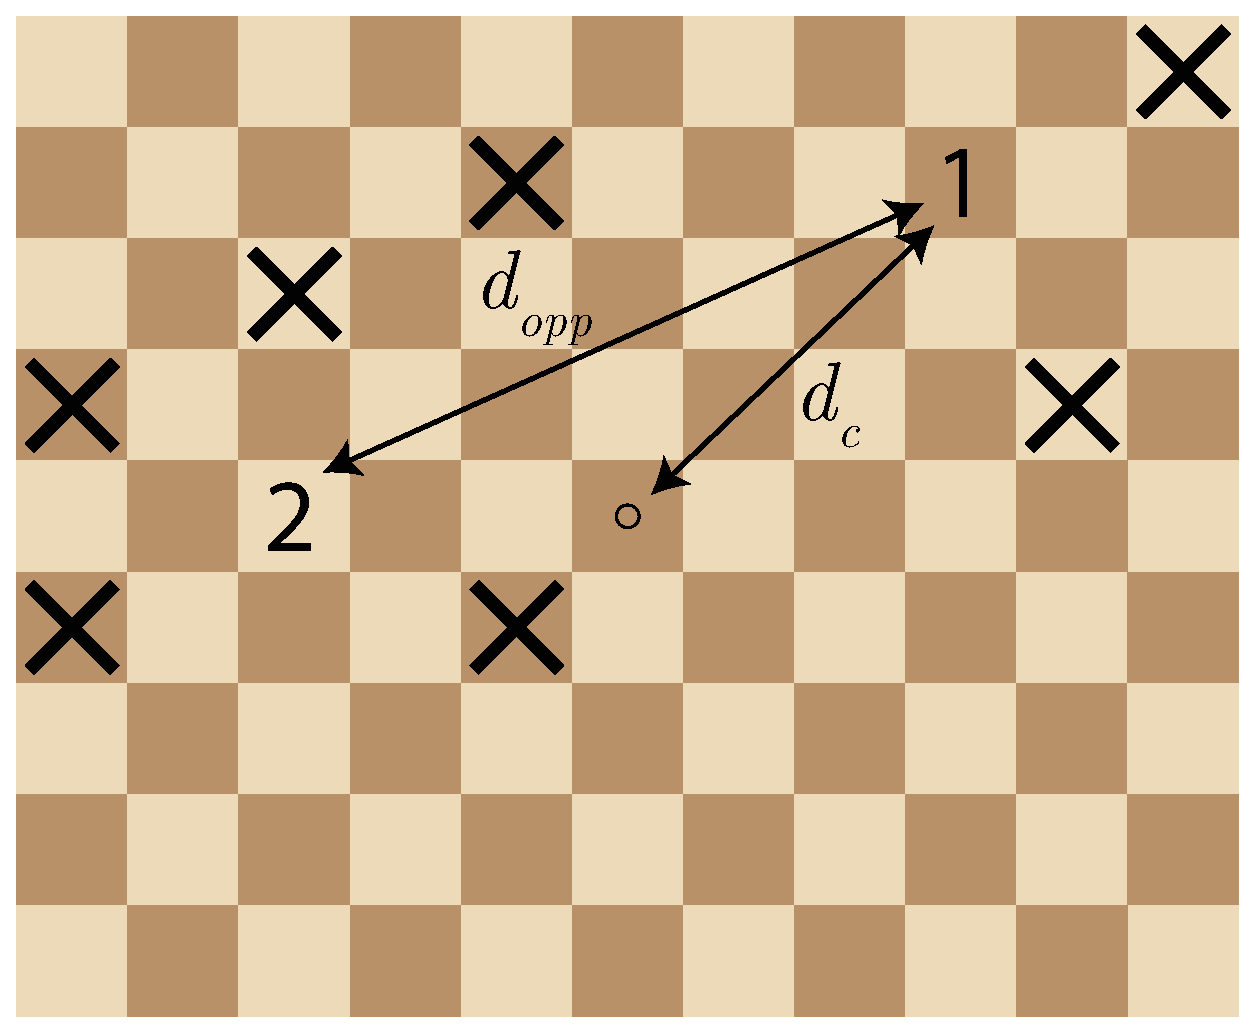
\includegraphics[width=\textwidth]{viz.eps}
 \caption{Snapshot of a game. The numbers 1 and 2 represent the position of the players. At the moment our player is Player 1. The crosses represent cells which the players previously visited and cannot visit anymore.}
 \label{fig:board}
\end{figure}

In Figure \ref{fig:board} it is depicted a snapshot of the game. The main purpose of this heuristic is to conquer the center of the board and avoid to move towards the edges of the board in which the number of moves can be limited (since the "pacman move" is not allowed).

The heuristic can be computed for every action can be computed with the following formula:
\begin{equation}
	\argmin_{a \in Actions(s)} \begin{cases}
		M d_c^2(\ell_{opp} - \ell_{own}) & \text{if} \;\; \ell_{opp} > \ell_{own}\\
		(d_c + d_{opp})^2 * max \{ 1, \ell_{own} - \ell_{opp}\} & \text{if} \;\; \ell_{opp} < \ell_{own}\\
	\end{cases}
\end{equation}

where $M$ (as in the big-M) is an upper-bound to the heuristic and represent a very high cost, $\ell_{opp}$ represent the liberties of the opponent, $\ell_{own}$ the liberties of the controlled player, $d_c$ the distance of the player from the center and $d_{opp}$ the distance between the players.

In other words, for all the actions available at the move $s$ the heuristic is computed in the following way:
\begin{itemize}
	\item If the number of liberties of the opponent is greater of the ones of the controlled player, then a very high number is assigned to avoid choosing that action. In case of parity, the action which keeps the player more in the center is preferred.
	\item If instead the controlled player has more liberties then, the actions with the lowest possible sum of $d_c$ and $d_{opp}$ is chosen. In case of very similar distances the ones with more liberties is preferred.
\end{itemize}
Using this heuristic the player tries to always stay between the opponent and the center.

\section{Algorithm}
The algorithm used to select the next action depends on the number of the movement and how fare we are in the game. If the game has just started a greedy approach, using the presented heuristic, is preferred in order to not having to deal with a large search space. In the endgame (after 45 moves) an alpha-beta pruning approach is preferred with a depth of $6$. Since in the endgame the branching factor is close to $1$ even if the cut-off is set at $150ms$ the $\alpha\beta$ algorithm is still able to find a solution. 

For this case search speed matters more than accuracy in the first part of the game while the opposite is true at the end of the game.

\section{Results}
In order to evaluate the efficiency of the proposed approach, a benchmark comparing the presented approach ($\alpha\beta + heu$) against players that implement different scenarios is here discussed. As it can be seen in Table \ref{result} the presented approach outperforms the Minimax algorithm and is able to win matches against the other players which implement a random, greedy or minimax approach.


\begin{table}[tb]
\centering
\begin{tabular}{|c|c|c|c|c|}
\hline
 & Random & Greedy & Minimax & $\alpha\beta+heu$ \\ \hline
Random & 50\% & 30\% & 5\% & 5\% \\ \hline
Greedy & 70\% & 50\% & 20\% & 15\% \\ \hline
Minimax & 95\% & 80\% & 50\% & 40\% \\ \hline
$\alpha\beta + heu$ & \textbf{95\%} & \textbf{85\%} & \textbf{60\%} & \textbf{50\%} \\ \hline
\end{tabular}
\caption{\label{result}Results of the matches between different players. Rows represent Player 1 and Columns Player 2. The percentage in the cells represent the times in which Player 1 won against Player 2. The tests were performed enabling the flag \texttt{fair\_matches}}
\end{table}


\end{document}
